\chapter{Transport coefficients in the conformal window}

Gauge theories with a nontrivial infrared (IR) fixed point are important in the context of model building Beyond the Standard Model \cite{Sannino:2008ha}. These theories are characterised by scale invariance in the infrared and, in the case of four space-time dimensions, they are invariant under the larger group of conformal transformations. For this reason, the region in theory space, parametrised by the number of colours ($N$) and fermion flavours ($N_f$), such that a nontrivial IR fixed point exists, is called conformal window.
Substantial effort has been taken in studying the properties of theories in the conformal window, both perturbatively and via lattice simulations (\emph{references?}). In this chapter, we present a study of the transport coefficients of theories in the perturbative conformal window, which has been published in \cite{Toniato:2016twr}.
The chapter is organised as follows: we start by introducing the conformal window and the definition of the transport coefficients under analysis. We then briefly sketch the method used by the authors of \cite{Arnold:2000dr} for calculating the transport coefficients of a gauge theory coupled to fermions. Finally, we present the results obtained by applying the perturbative results of \cite{Arnold:2000dr} to theories in the conformal window. 

%%%%%%%%%%%%%%%%%%%%%%%%%%%%%%%%%%%%%%%%%%%%%%%%%%%%%%

\section{The conformal window}
\label{ conformal_window}

We consider a non-Abelian gauge theory, with gauge group SU($N$) and $N_f$ fermions in the representation $r$. The two-loop beta function for the gauge coupling $g$ is given by:

 \begin{equation}
 \beta (g) = - \frac{\beta_0}{(4\pi)^2} g^3 - \frac{\beta_1}{(4\pi)^4} g^5 + \mathcal{O}(g^{7}) \; ,
 \label{beta_f}
 \end{equation}
%
with

 \begin{align}
\beta_0 &= \frac{11}{3} C_2[G] - \frac{4}{3} T[r] N_f\; , \\
\beta_1 &= \frac{34}{3} C_2^2[G] - \left ( \frac{20}{3} C_2[G] + 4 C_2[r] \right ) T[r] N_f\; ,
\end{align}
%
where $G$ denotes the adjoint representation. The definition of the group factors $C_2$, $T$ and $d$ can be found in appendix \ref{SUN_generators}. If $\beta_0 > 0$, the theory is asymptotically free, i.e. $g=0$ is an ultraviolet(UV)-stable fixed point of the renormalisation group (RG) flow. This happens provided the number of fermions is smaller than the upper limit:

\begin{equation}
N_f^{AF} = \frac{11}{4} \frac{C_2[G]}{T[r]} \: .
\end{equation}
%
The number of flavours and colours can be chosen such that $\beta_0>0$ and $\beta_1<0$. In this case there exists an additional zero of the beta function:

\begin{equation}
g^* = -(4 \pi)^2 \frac{\beta_0}{\beta_1} \: .
\end{equation}
%
This is an IR-stable fixed point, which can be studied in perturbation theory in case $g^*$ is small \cite{Banks:1981nn}. In particular, $g^*$ goes to zero in the limit $N_f \to N_f^{AF}$. If $g^*$ is small, the theory remains perturbative along the whole RG flow, from the UV, where it is dominated by the asymptotically free fixed point $g=0$, down to the IR. If $g^*$ is not small enough, then one has to consider higher-order terms in the beta function \ref{beta_f}, and eventually, when $g^*$ leaves the perturbative regime, apply non-perturbative methods such as lattice simulations. In theory space, parametrised by $N$ and $N_f$, the upper boundary of the conformal window for every fixed $N$ is given by $N_f = N_f^{AF}$, while the lower boundary is yet to be found via non-perturbative methods, since the value of $g^*$ increases with decreasing $N_f$.


\begin{figure}[h!]
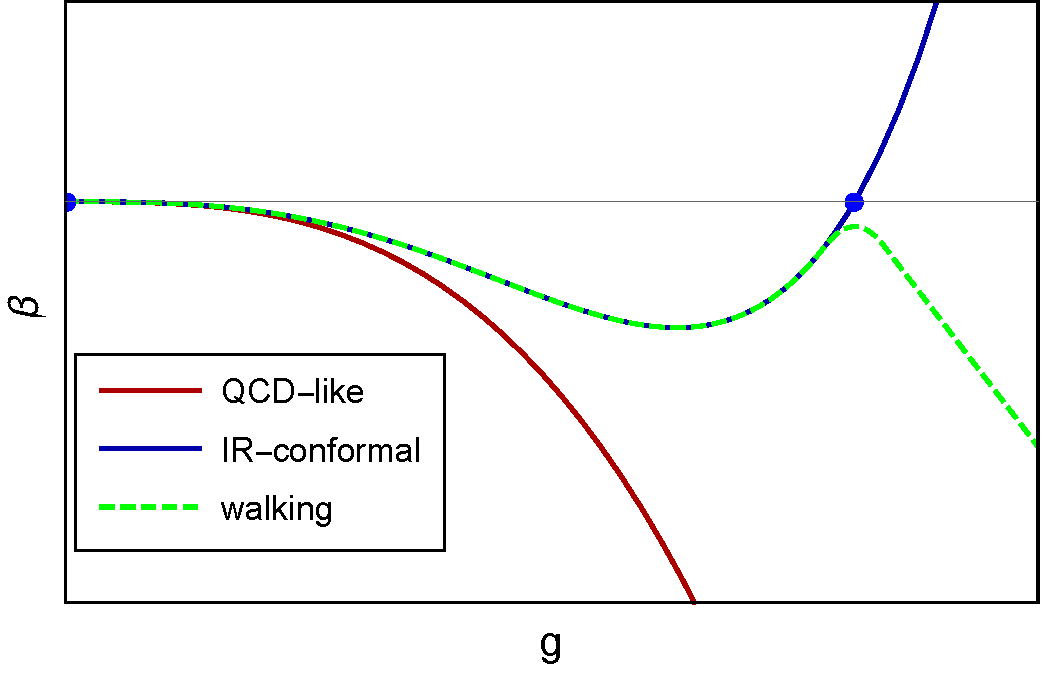
\includegraphics[width=0.5\textwidth]{pics/beta_walking}~~~
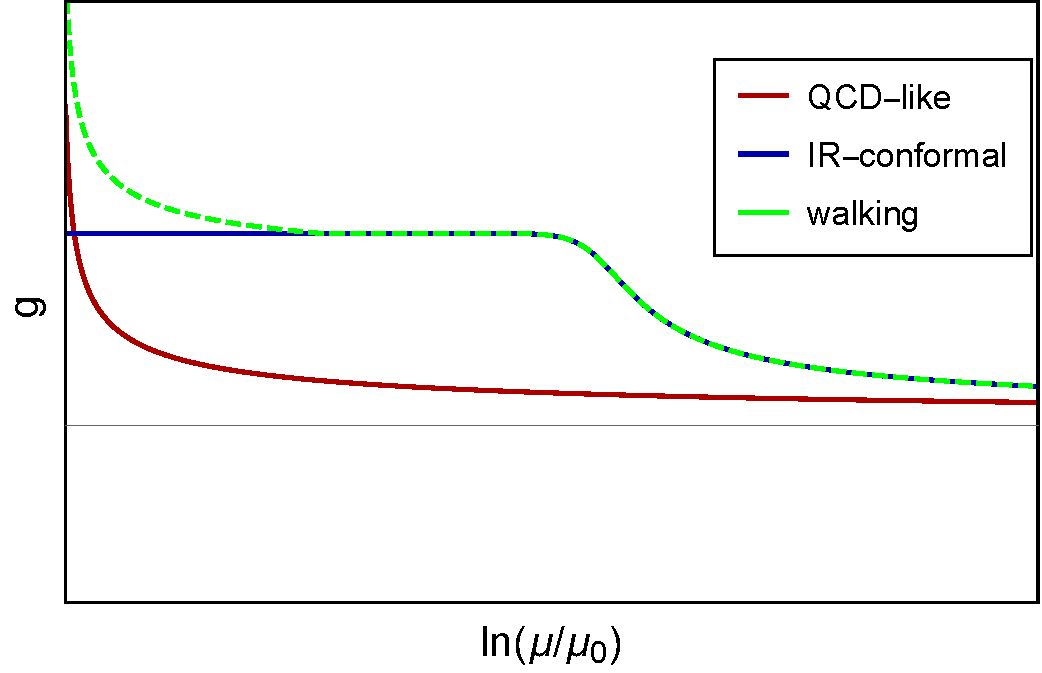
\includegraphics[width=0.5\textwidth]{pics/g_walking}
\caption{Beta function (left panel) and gauge coupling (right panel) for three different kinds of theories: a QCD-like theory (red line), a theory in the conformal window (blue line) and a theory with walking gauge coupling (green dashed line). In the right panel, the gauge coupling is plotted as a function of the energy scale $\mu$ over some reference scale $\mu_0$.} 
\label{walking}
\end{figure}


Figure \ref{walking} shows three different regimes of the beta function, and the related running of the gauge coupling. The first one (red line) characterises a QCD-like theory. The beta function has one single zero at $g=0$, and is negative for all other values of $g$. In this case, the coupling goes to zero in the UV (asymptotic freedom) and grows when moving towards the IR, until it diverges at some finite energy scale. This theory displays spontaneous chiral symmetry breaking in the IR. The second regime (blue line) characterises a theory in the conformal window. The beta function has two zeros, $g=0$ and $g=g^*$, and is negative in between. The gauge coupling goes to zero in the UV, and stabilises at the fixed point value $g=g^*$ in the IR. This theory is characterised by scale invariance in the IR, and does not display spontaneous chiral symmetry breaking. The third regime (green dashed line) is associated to "walking" dynamics. It is reasonable to assume that, close to the lower boundary of the conformal window, theories with an approximate IR fixed point can be found. Their beta function is very similar to the one of theories in the conformal window, with the difference that it gets very close to zero at $g\simeq g^*$, without actually reaching a fixed point, and then assumes a QCD-like behaviour for larger values of $g$. In this theory the gauge coupling goes to zero in the UV, then stabilises at an approximately constant value for a wide range of energies, and finally diverges at a finite energy scale, thus triggering chiral symmetry breaking. Theories with walking gauge coupling are very important in the context of composite Higgs models, as discussed in section \ref{partial_comp}. In fact these theories show an approximate conformal behaviour, which can lead to a nice separation of scales and good scaling properties of composite operators, and at the same time break chiral symmetry, which is a necessary ingredient in composite Higgs models.
Lattice simulations can be used in order to find out whether a theory is in one of the three regimes shown in figure \ref{walking}, see for example \cite{Hietanen:2008mr,Hansen:2017ejh}.

Here we consider theories in the perturbative conformal window, i.e. $N_f \lesssim N_f^{AF}$, and we study their sheer viscosity and fermion number diffusion coefficient by applying the perturbative results obtained in \cite{Arnold:2000dr}.

%REMEMBER TO JUSTIFY THE FACT THAT THE NUMBER OF FLAVOURS IS TREATED LIKE A CONTINUOUS PARAMETER!

%%%%%%%%%%%%%%%%%%%%%%%%%%%%%%%%%%%%%%%%%%%%%%%%%%%%%%

\section{Transport coefficients}

Transport coefficients characterise the response of a fluid to small deviations from thermodynamic equilibrium. The transport coefficients considered in our study are viscosity and diffusion coefficients. Viscosity describes the response to spacial variations of the flow velocity, in the presence of dissipative phenomena (internal friction). Diffusion coefficients describe the evolution of the density of conserved charges, when the charge concentration is not uniform over the fluid. In this section we introduce the equations of motion of a viscous fluid and the diffusion equation, which provide the definitions of the transport coefficients under analysis.

\subsection{Viscosity}

In this derivation we follow the lines of \cite{landau2013fluid}. We start by considering the motion of an ideal fluid, which is described by the continuity equation:

\begin{equation}
\partial_t \rho + \partial_i (\rho v_i) = 0 \: ,
\end{equation}
%
and Euler's equation (given here in component form):

\begin{equation}
\partial_t v_i +  v_j \partial_j v_i = -\frac{1}{\rho} \partial_i p \: ,
\end{equation}
%
where time is denoted by $t$, spacial coordinates by $x_i$ ($i=1,2,3$), the fluid mass density by $\rho$, the flow velocity components by $v_i$,  and the pressure by $p$. Sums over repeated indices are understood. Euler's equation can be rewritten as:

\begin{equation}
\partial_t (\rho v_i) = - \partial_j \Pi_{ij} \: ,
\label{Euler}
\end{equation}
%
where the symmetric tensor $\Pi_{ij} = p \delta_{ij} + \rho v_i v_j$ represents the flux density of the momentum component $i$ in all possible directions $j$. The momentum transfer described by the tensor $\Pi_{ij}$ is reversible, and it is due to the mechanical transport of volumes of fluid and to pressure forces acting in the fluid. The motion of a viscous fluid is characterised by an extra, irreversible, transfer of momentum, occurring from points where the flow velocity is large to points where it is low.
In the case of a viscous fluid, the tensor $\Pi_{ij}$ can be parametrised as:

\begin{equation}
\Pi_{ij} = p \delta_{ij} + \rho v_i v_j - \sigma_{ik} \: ,
\end{equation}
%
where $-\sigma_{ik}$ is the contribution due to internal friction. Always following \cite{landau2013fluid}, we notice that $\sigma_{ik}$ must depend on the spacial derivatives of the flow velocity, since internal friction occurs only when different layers of fluid move with respect to each other, and must vanish when the flow velocity is constant in space. Moreover, $\sigma_{ij}$
must vanish when the fluid is in uniform rotational motion, because in this case there is no relative motion between different layers of fluid. The flow velocity of a uniformly rotating fluid is expressed as: $\vec v = \vec \Omega \times \vec r$, $\vec r$ being the distance from the centre of rotation and $\vec \Omega$ the constant angular velocity. If the velocity gradients are small, we may assume that $\sigma_{ik}$ is a linear function of the first derivatives of the flow velocity. The most general function of this sort, which vanishes in case $\vec v = \mathrm{constant}$, or $\vec v = \vec \Omega \times \vec r$, is:

\begin{equation}
\sigma_{ij} = \eta \biggl( \partial_i v_j + \partial_j v_i -\frac{2}{3} \delta_{ij} \partial_k v_k \biggr) + \zeta \delta_{ij} \partial_{k} v_k \: ,
\label{viscosity_classical}
\end{equation}
%
where the coefficient $\eta$ is the shear viscosity and $\zeta$ the bulk viscosity. The terms in equation \ref{viscosity_classical} are organised so that the expression in parentheses vanishes when traced over $i$ and $j$. To conclude, for a viscous fluid

\begin{equation}
\Pi_{ij} = p \delta_{ij} + \rho v_i v_j - \eta \biggl( \partial_i v_j + \partial_j v_i -\frac{2}{3} \delta_{ij} \partial_k v_k \biggr) - \zeta \delta_{ij} \partial_{k} v_k \: ,
\label{Navier-Stokes}
\end{equation}
%
and Euler's equation is substituted by the Navier-Stokes equation, obtained by inserting \ref{Navier-Stokes} in \ref{Euler}.


Relativistic fluid equations describe a fluid whose flow velocity is relativistic, or whose microscopical components move at relativistic speed. In order to derive them, we introduce the energy-momentum tensor $T^{\mu\nu}$ of the relativistic fluid. The component $T^{00}$ is the fluid energy density, $T^{i0} = T^{0i}$ is the momentum component density (equal to the energy flux density), and $T^{ij}$ the momentum flux density, analogue to the non-relativistic $\Pi_{ij}$. The equations of motion

\begin{equation}
\partial_{\mu} T^{\mu\nu} = 0
\end{equation}
%
express the conservation of energy and momentum in the fluid.
We start by defining $T^{\mu\nu}$ for an ideal fluid in the local rest frame. In the local rest frame, the momentum density is zero ($T^{0i} = 0$), and the force exerted by the fluid on some surface is the same in all directions, and always perpendicular to the surface. The $i$-th component of the force exerted on an infinitesimal surface $\mathrm{d} \hat \Sigma = \abs{\mathrm{d}\Sigma} \: \hat n$ is given by:  $T^{ij} \mathrm{d} \hat \Sigma^j $, where $\hat n$ is the normal to the surface. It follows from the above argument that $T^{ij} \mathrm{d} \hat \Sigma^j = p \: \mathrm{d} \hat \Sigma^i $, and therefore $T^{ij} = \delta^{ij} p$. Consequently, in the local rest frame:
 
 
 \begin{equation}
 (T^{\mu\nu}) =
 \begin{pmatrix}
 e & 0 & 0 & 0 \\
 0 & p & 0 & 0 \\
 0 & 0 & p & 0 \\
 0 & 0 & 0 & p \\
 \end{pmatrix} \: ,
 \label{T_rest_frame}
 \end{equation}
 %
 where $e$ is the energy density and $p$ the pressure.
 This expression can be generalised to a generic reference frame by introducing the fluid four-velocity $u^{\mu}$, which in the local rest frame is given by $u^0 =1$, $u^i =0$, and in a frame in which the fluid element moves with velocity $\vec v$ by $u^0 = 1/\sqrt{1-v^2}$, $u^i = v^i/\sqrt{1-v^2}$. In a generic frame, $T^{\mu\nu}$ is expressed as:
 
 \begin{equation}
 T^{\mu\nu} = (e+p) u^{\mu} u^{\nu} - p \: \eta^{\mu\nu} \: ,
 \label{Tmunu}
 \end{equation}
 %
 where $\eta_{\mu\nu}$ is Minkowski metric. Equation \ref{T_rest_frame} is recovered by fixing $u^0 =1$, $u^i =0$.
In the presence of internal friction, further terms must be added to the energy momentum tensor \ref{Tmunu}. In the local rest frame, the spatial components of the energy momentum tensor of a viscous relativistic fluid are given by:

\begin{equation}
T_{ij} = p \delta_{ij} - \eta \biggl( \partial_i u_j +\partial_j u_i - \frac{2}{3} \delta_{ij} \partial_k u_k \biggr) - \zeta \delta_{ij} \partial_k u_k \: ,
\label{viscosity_def}
\end{equation}
%
which reduce to \ref{Navier-Stokes} in the non-relativistic limit $\abs{v} \ll 1$. Equation \ref{viscosity_def} may be regarded as the definition of the shear and bulk viscosities of a relativistic fluid.
 
 \subsection{Diffusion coefficient}
 
We have seen that the equations of motion of a relativistic fluid express the conservation of energy and momentum. Further conservation equations exist for any other conserved quantity. We consider here the case of a conserved particle number density. The conservation equation takes the form:
 
 \begin{equation}
 \partial_{\mu} j^{\mu} = 0 \: ,
 \label{cons_density}
 \end{equation}
 %
 where $j^{\mu} = n \: u^{\mu}$, $u^{\mu}$ being the fluid four-velocity and $n$ the particle number density in the local rest frame.
 The diffusion equation:
 
 \begin{equation}
 \partial_t n = D \Laplace n \: ,
 \label{diffusion_eq}
 \end{equation}
 %
 where $\Laplace = \partial_i \partial^i$, describes the evolution of the number density $n$, when $n$ is low and not uniform over the fluid. In this case, the number density flux can be expressed, in the local rest frame, as:
 
\begin{equation}
j^i = - D \partial^i n \: ,
\label{diffusion_current}
\end{equation}
%
which, in combination with the conservation law \ref{cons_density}, implies the diffusion equation \ref{diffusion_eq}. The coefficient $D$ is known as diffusion coefficient. Equations of the form \ref{diffusion_eq}, \ref{diffusion_current} describe for example the evolution of the concentration $c$ of the solute in a weak solution ($c \ll 1$) \cite{landau2013fluid}, or the density of particles undergoing Brownian motion. It will be shown in the following that conserved currents related to global flavour symmetries in a hot gauge theory evolve diffusively.


%%%%%%%%%%%%%%%%%%%%%%%%%%%%%%%%%%%%%%%%%%%%%%%%%%%%%%

\section{Transport coefficients of a hot gauge theory: kinetic approach}

The equilibrium state of a high temperature quantum field theory can be described as a relativistic fluid. Transport coefficients can in principle be computed, based on the dynamics of the underlying microscopic theory.
This is what the authors of \cite{Arnold:2000dr,Arnold:2003zc} did in the case of a weakly coupled , high temperature gauge theory, both in a leading-log approximation \cite{Arnold:2000dr} and in a full leading order treatment \cite{Arnold:2003zc}.
In this section, without aiming at a complete description, we would like to sketch the method used in these works to compute the transport coefficients. The analytic results given in \cite{Arnold:2000dr}, together with the coefficients in table \ref{AB}, are the basis for our study of transport coefficients in the perturbative conformal window.

In \cite{Arnold:2000dr,Arnold:2003zc}, a finite-temperature gauge theory coupled to fermions is considered, under the assumption that the gauge coupling at the scale of the temperature is weak: $g(T) \ll 1$.

\subsection{Leading-log and next-to-leading-log results}

    \begin{table}[h!]
\begin{center}
    %\begin{minipage}{3.8in}
    \begin{tabular}{c||ccc }
    $N_f$ & $ \quad A$ & $\quad B $ &   \\
    \hline \hline
    $ 6 $ & \quad 2.918 & \quad 3.064   \\
        $14$ &\quad 2.878 &\quad 3.135  \\
        $15$ & \quad 2.873 & \quad 3.172 \\
        $16$ & \quad 2.869  & \quad 3.176 \\
    $16.25$ & \quad 2.867 & \quad 3.177
    \end{tabular}
    %\end{minipage}
    \end{center}
\caption{Values of the coefficients $A$ and $B$ \cite{privcommGDM}
appearing in the next-to-leading-log expressions of the shear viscosity and the fermion-number diffusion coefficient, 
for $N = 3$ and different values of $N_f$.}
\label{AB}
    \end{table}


%%%%%%%%%%%%%%%%%%%%%%%%%%%%%%%%%%%%%%%%%%%%%%%%%%%%%%

\section{Application to theories in the conformal window}

%%%%%%%%%%%%%%%%%%%%%%%%%%%%%%%%%%%%%%%%%%%%%%%%%%%%%%
